\subsubsection{Bench Press}

The bench press is an upper body movement in which the lifter will lie on a bench parallel to the ground, with the barbell above the lifter on a rack. The lifter will grip the barbell with their hands. The barbell is unracked and the lifter must allow the bar to descend onto their chest by bending their elbows and shoulders. When the bar touches the lifters chest, they must push vertically on the bar to lock out their elbows. A bench press is considered successful if the barbell touches the chest, and the elbows are successfully locked upon completion. Figure~\ref{fig:bench_stages} shows an example of a bench press.

\begin{figure}[H]
    \centering
    \subfigure[Begin]{
            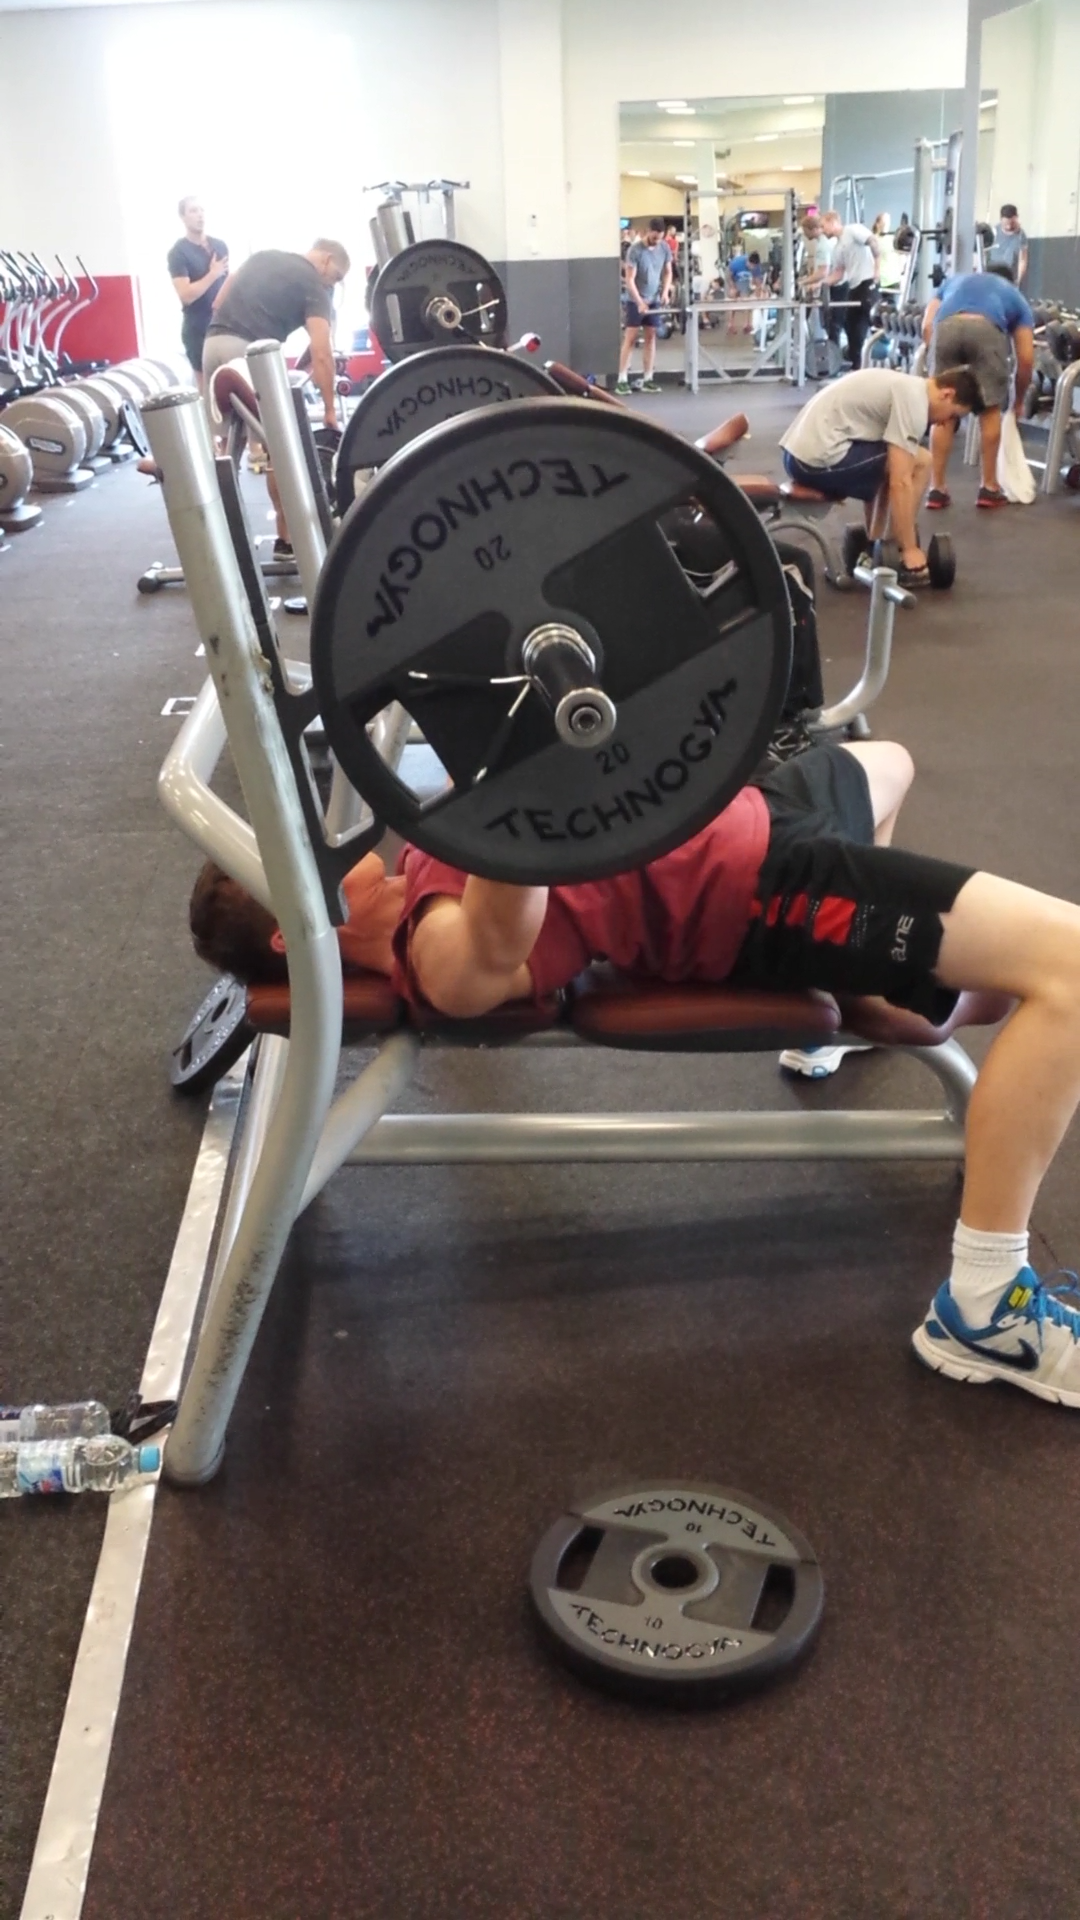
\includegraphics[height=3cm]{intro/images/bench_start}
    }
    \subfigure[Middle]{
            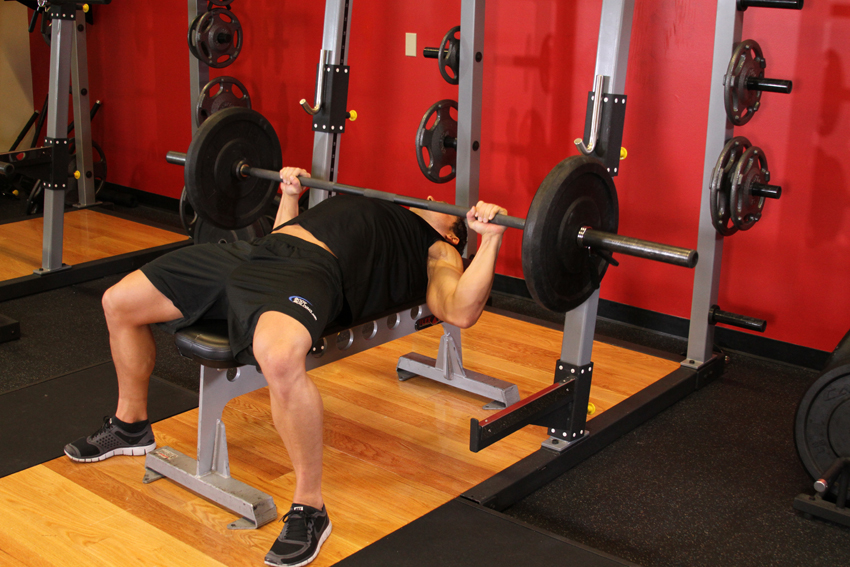
\includegraphics[height=3cm]{intro/images/bench_middle}
    }
    \subfigure[End]{
            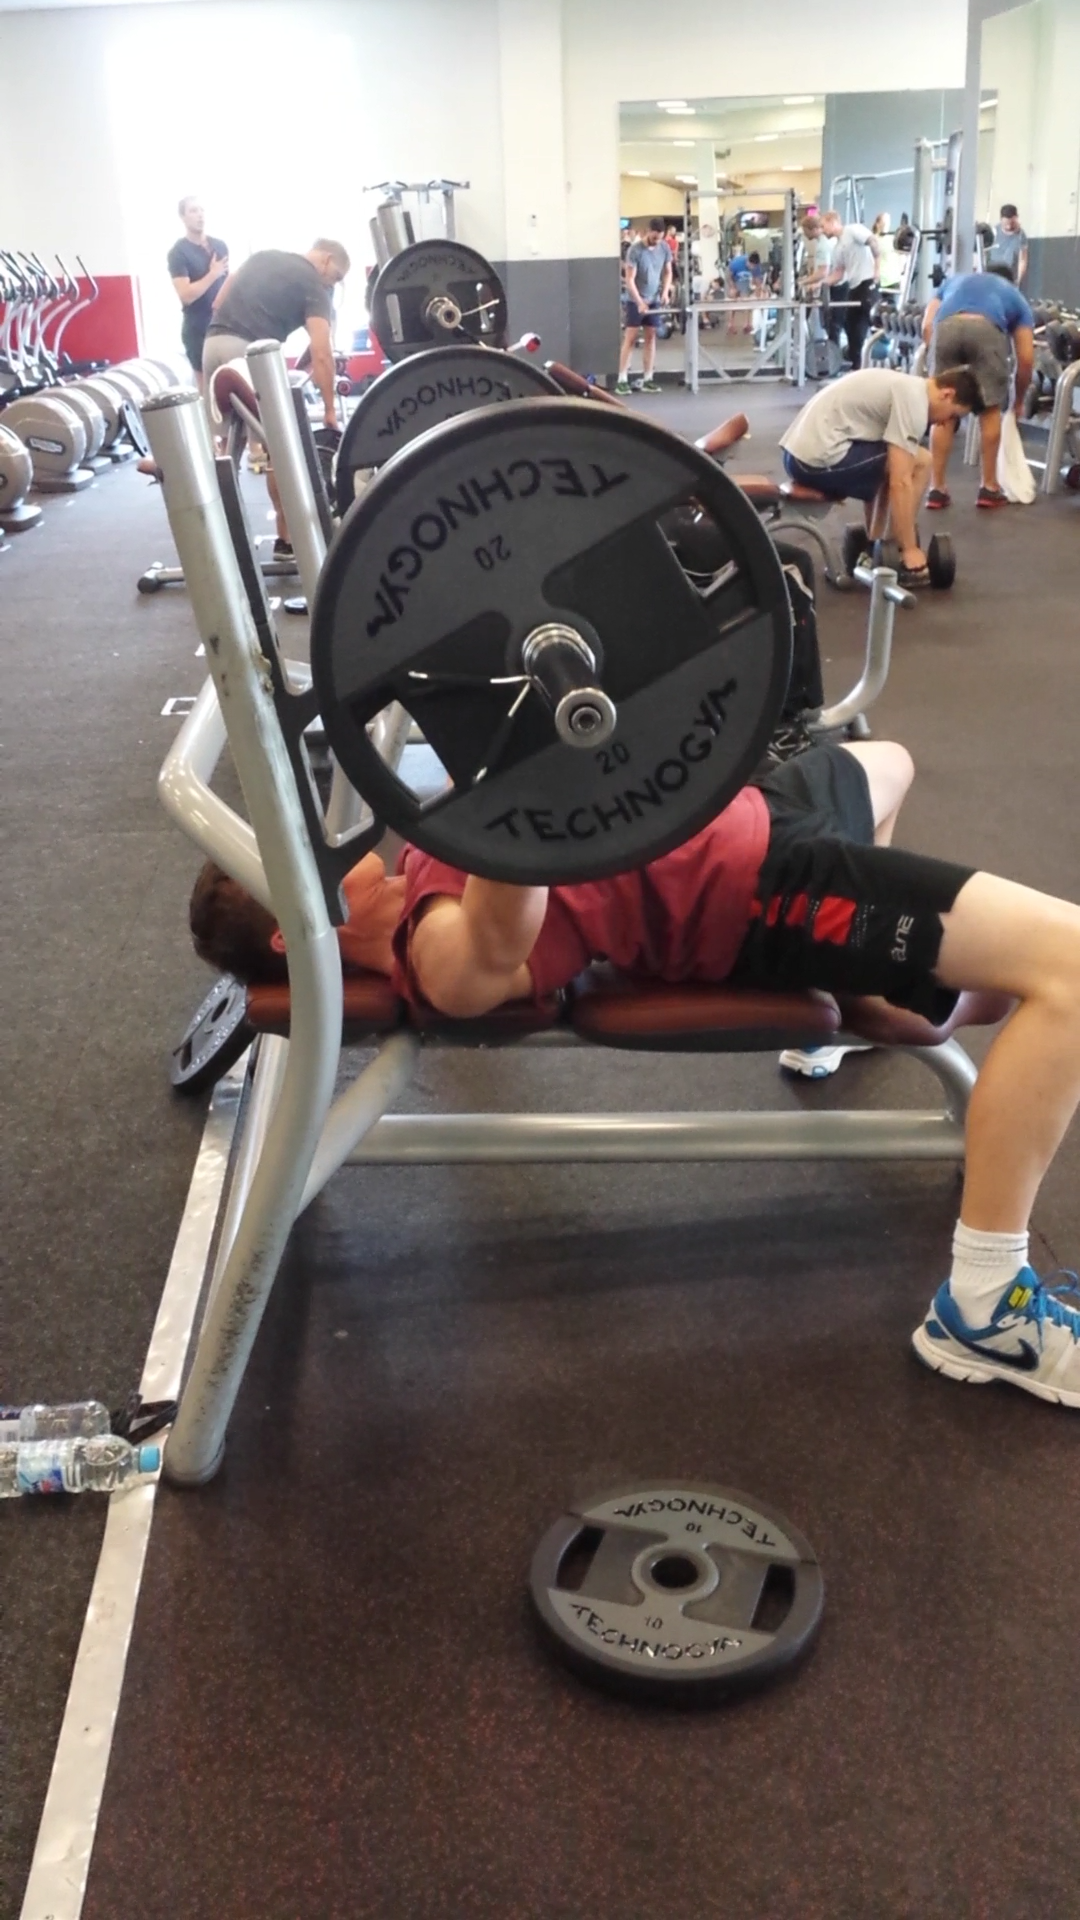
\includegraphics[height=3cm]{intro/images/bench_start}
    }
\caption{The stages of a bench press}
\label{fig:bench_stages}
\end{figure}

The International Powerlifting Federation regulations\cite{ipf} state that during the bench press, the body position of the lifter must not change, ie. there must be no raising movement of the head, shoulders or buttocks.